\documentclass[journal]{./IEEE/IEEEtran}
\usepackage{cite,graphicx,ragged2e}
\newcommand{\tab} [1][0.5cm]{\hspace*{#1}}

\newcommand{\SPTITLE}{I.C.S: Interactive Coding for Students, a 3D Educational Programming Game}
\newcommand{\ADVISEE}{Vaughn Victor A. Chua}
\newcommand{\ADVISER}{Toni-Jan Keith Monserrat}

\newcommand{\BSCS}{Bachelor of Science in Computer Science}
\newcommand{\ICS}{Institute of Computer Science}
\newcommand{\UPLB}{University of the Philippines Los Ba\~{n}os}
%\newcommand{\REMARK}{\thanks{Presented to the Faculty of the \ICS, \UPLB\
   %                          in partial fulfillment of the requirements
      %                       for the Degree of \BSCS}}
        
\markboth{CMSC 190 Special Problem, \ICS}{}
\title{\SPTITLE}
\author{\ADVISEE~and~\ADVISER%
%\REMARK
}


%\pubid{\copyright~2017~ICS \UPLB}

%%%%%%%%%%%%%%%%%%%%%%%%%%%%%%%%%%%%%%%%%%%%%%%%%%%%%%%%%%%%%%%%%%%%%%%%%%

\begin{document}

% TITLE
\maketitle

% ABSTRACT
\begin{justify}
\begin{abstract}
\thispagestyle{empty}
In this study, we created a 3D educational game that teaches players basic programming commands. This study provided the necessary aid of students who are willing to learn programming or do not have any idea how the basic programming commands work. Respondents, both without any background in programming and with background, tested the game and answered a survey in which they were asked if they have learned anything in the game. The results provided that upon finishing the game, the players grasped the idea of how to think when programming and how the basic programming commands work. The study can be a medium for other developers to create more educational games for students and inspire people to learn programming even if it is not their major. Lastly, this study can be a gateway for aspiring students in expanding their knowledge in creating teaching methods on how they can help their fellow students learn not just in programming but in other fields as well.
\end{abstract}
% INTRODUCTION
\section{\textbf{Introduction}} Nowadays, professors either use a board or use slide presentations to teach. These techniques have obvious limitations to them. Students tend to only listen and write but there is no guarantee that they will learn. One way to improve the student's learning experience is by integrating 3-D tools. Those tools are in the form of a simulation or a game. But, not all games or simulations are accessible offline. The problem in using the common way of teaching is that it lacks student interaction. In Computer Science 11 or CMSC 11, there is an introductory exercise wherein students play an educational game for programming. Implementing educational games will help the students to understand further the topics that are being discussed, not only will it help the students with further understanding the lessons, it will also give them entertainment at the same time which makes them focus more.\newline
\tab The solution to the problem will be to create and implement a 3D educational programming game that tackles the use of basic commands that are commonly used when coding. This is intended for students who are not yet knowledgeable of how to program, or anyone who is interested in learning how to program. The objective of this study is to make the students learn basic commands in programming and the proper thinking when coding. The game will be made using Blender's Game Engine and will be deployed as an independent application for computers or android smartphones which can be played without relying on internet connections. The game will have a user-friendly experience to users without knowledge in programming and teaches them on how to code will be able to understand the instructions completely. In the ICS community, the game can be used as a learning tool in teaching the basics of programming and could attract more non computer science students to take any computer science courses as an elective.

%Related Work
\section{\textbf{Related Work}}The following will tackle the works of different authors in relation to this study. In the article of \cite{educ_game}, their research found that games can be used as a tool for better understanding the lessons. It is also said that in their experiment, the number of students who got an “A” grade increased by 7 percent with the use of an educational game. \cite{cross_plat}, their study is about the Cross-platform Application Development Using Unity Game Engine. 
In this, the authors talked about how Unity3D is being used as a game engine and its power to create and present games to different platforms including Android, iOS, Windows etc… In the end of their study, they created an Air Hockey game in which it can be ported to different platforms. In \cite{cross_plat}, the author stated that``The type of business model depends on the ability to record, analyze and interpret analytics and metrics to finesse the user experience and plan future iterations of a product to ensure a high level of user retention and monetization”\cite{engagement}.  One article by \cite{kids} showed that there are already 
educational games that are existing on the internet and one of those is Code.org’s Hour of Code game however an internet connection is needed for students to be playable and also it is made in 2D. 
In the study of \cite{performance}, their experiment showed that by creating an online educational game, the participants’ learning achievements, flow experience, learning attitudes have improved when they played the game.
According to \cite{virtual_reality}, a game called ``Second Life” has been created and its purpose is to educate the users of how the real world is like with the use of 3D technology. It is proven effective since the accounts that were created grew from two hundred thousand (2006) to four million (2007). A game has been developed by \cite{corgi} and is entitled ``Corgi Defence".
It is a puzzle game in which players are required to solve in the virtual reality world. The authors' conclusion is that the game is enjoyable however it is still being limited by the hardware in recognizing hand gestures.
	This paper uses Blender as its main game engine and being open-sourced, other people can create games as well. Many of the educational games that were made to teach programming are in 2D while the game created in this paper is 3D. The difference between the paper and the other studies is that this could be potentially be used as a regular learning tool for the students who want to learn basic programming codes without having the problem of a stable internet connection.


% MATERIALS AND METHODS
\section{\textbf{Methodology}}
Blender, an open-sourced technology, is used to create the game. \cite{blender} After developing the game, it is ported as an independent application ready to be used in computers. The game is lightweight which means it does not require heavy graphics card to be able to play it smoothly. Upon development, the game will be optimized and the core gameplay is based on the most optimized way of programming.

The step-by-step procedure will be as follows:\\
\\
1.)	\textit{Game Design} - This is the most important part of the development process because this is the main component on how the game will work from the beginning to the end. The design for this study's game is on a linear basis. Using the in-game objects, the player can solve various problems in the area so that he/she can move to another area. 
\\
\newline
2.)	\textit{Map Creation and Functionalities} - The map is 3D and for the functionalities, they are a mixture of Blender’s logic editor and are coded using the Python language. Coincidentally, this language is also the language being taught in CMSC 11 at the moment which means the students will understand the codes easily. \textit{See Fig. \ref{action}}\newline
\begin{figure}[ht]
   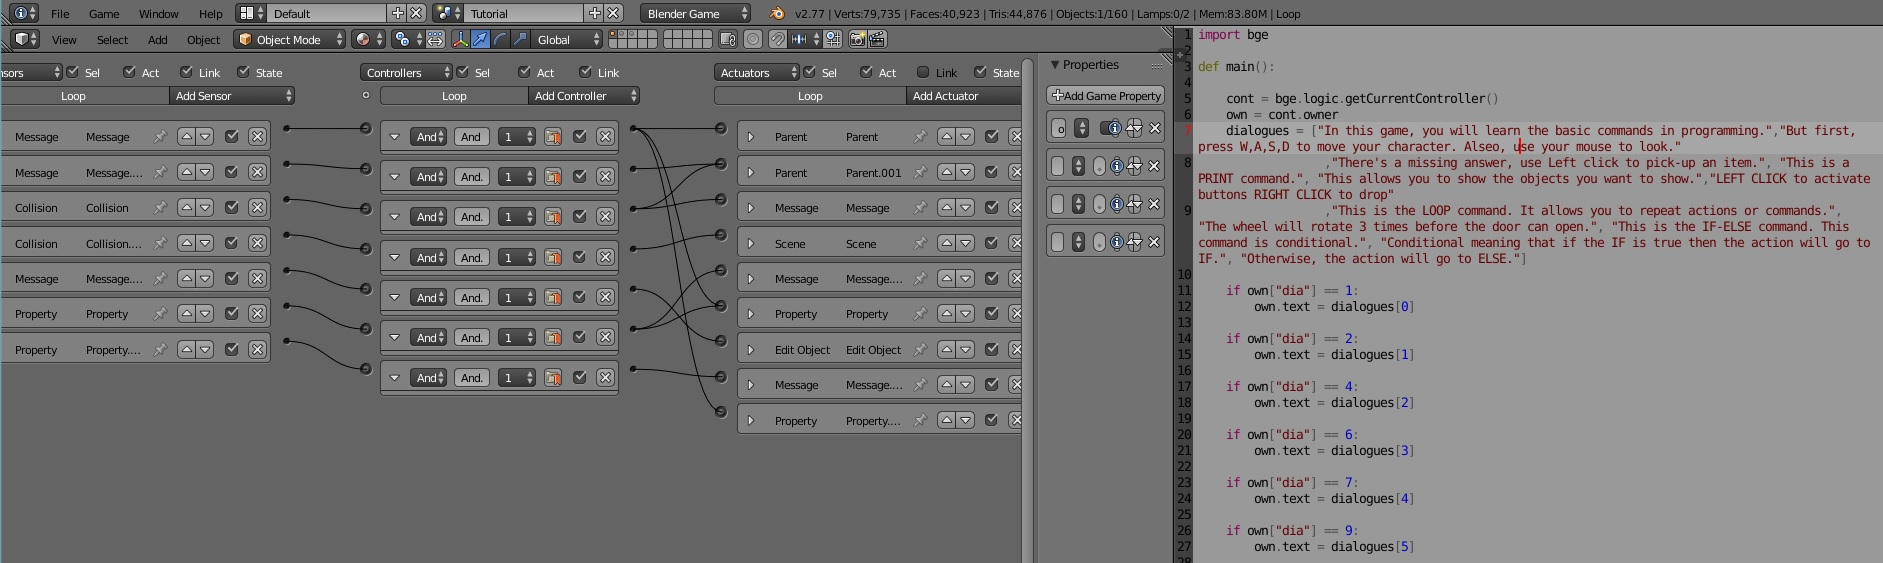
\includegraphics[width = 8.5cm]{images/actions}
   \caption{Functionalities for the character in the game}
   \label{action}
\end{figure}\newline 3.)	\textit{Player and Object Modelling} - Blender uses vectors and meshes for smooth modelling of 3D objects, the player along with the in-game objects will be modelled here and will be imported to the game engine. \textit{see Fig. \ref{model}}\\
\begin{figure}[ht]
   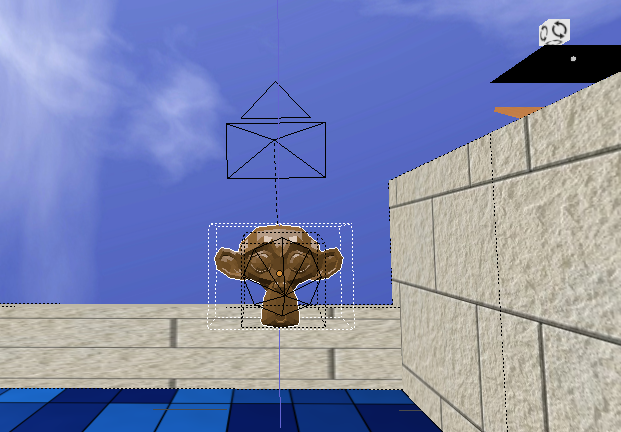
\includegraphics[width = 8.5cm]{images/model}
   \caption{Character Modelling}
   \label{model}
\end{figure}

4.)	\textit{Puzzle and Code Problem Creation} - \textit{see Fig. \ref{problem}} There is a tutorial level in which the players are taught of the basic controls in the game. Puzzles are created in a static manner which means problems are the same even if the player decides to restart the game. 
The interaction between the game and the user will be as follows:\newline
a.)	The user inputs or executes a command,\newline
b.)	The game receives the command and returns the correct action for the user input.\newline
c.)	Upon completing the task required in the level, the game lets the user to move to the next challenge of the game. \newline

\begin{figure}[ht]
   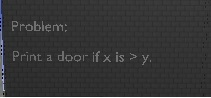
\includegraphics[width = 8.5cm]{images/problem}
   \caption{One of the problems to be solved inside the game}
   \label{problem}
\end{figure}

%Evaluation
\section{\textbf{Evaluation}}

The game was evaluated by checking the user’s level of enjoyment of the game, the level of difficulty of each puzzle or problem presented, the time that they finished the game and how well did they learn from it. The users that were picked to test the game will be divided into two groups of players; the first group of players were the ones knowledgeable of basic programming commands (7 players) while the other group are players that were complete beginners when it comes to programming (8 players). The users that were chosen are teenagers; they can be a high school student or a college student. For this study, there were 15 college students and no High Schol student of different courses such as (Biology, Forestry, MST, Engineering, Human Ecology, ABT) and only 1 was a Computer Science student. Also, the users were asked if they want to repeat the game and if they have suggestions for improving the game. After recording the feedbacks, the researcher were able to point out where to improve the game and what other factors the game lacks. We recruited 15 testers that will be testing the game.

% RESULTS
\section{\textbf{Results}}
After the participants played the game, the researcher then let them answer a survey and the important questions with their responses as follows:\newline \newline
1.)	How well were the instructions inside the game explained? \textit{See Fig. 4}\newline
-Not clear (3 people)\newline
-Average (7 people)\newline
-Clear (5 people)
\begin{figure}[ht]
   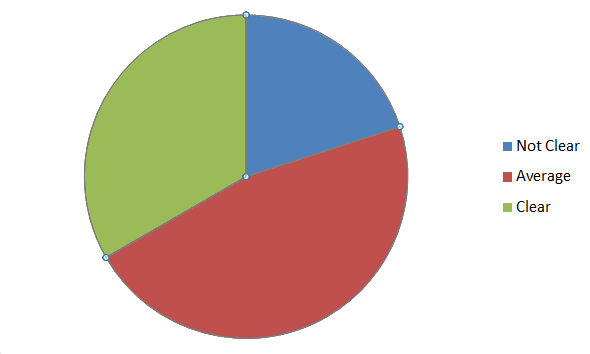
\includegraphics[width = 8.5cm]{images/pie}
   \caption{Pie Chart for the clarity of instructions for the testers}
   \label{4}
\end{figure}
\newline
\newline
\newline
2.) From 1-10, How did the aesthetics of the game appeal to you? \textit{See Fig.5}\newline
-An average of 5.93 has been given.
\begin{figure}[ht]
   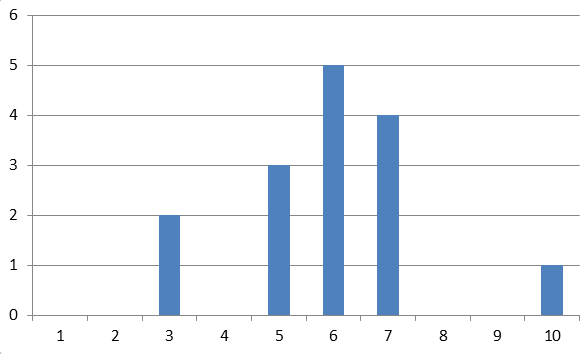
\includegraphics[width = 8.5cm]{images/bar3}
   \caption{Bar Graph of the aesthitics in the game for the testers}
   \label{5}
\end{figure}
\newline
3.) From 1-10, how well did you learn the basic commands in programming? \textit{See Fig. 6}\newline
-Respondents with no background (7.5 in average)\newline
-Respondents with background (8.43 in average) \newline
\begin{figure}[ht]
   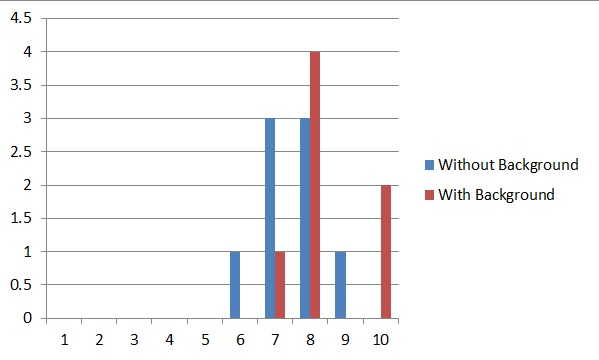
\includegraphics[width = 8.5cm,height = 4.5cm]{images/bargraph}
   \caption{Bar Graph for the rate of comprehension in basic commands in programming of testers.}
   \label{1}
\end{figure}
\\
4.) From 1-10, rate the level of your enjoyment on the game. \textit{See Fig.7} \newline
-An average of 7.4 has been given. \newline
\begin{figure}[ht]
   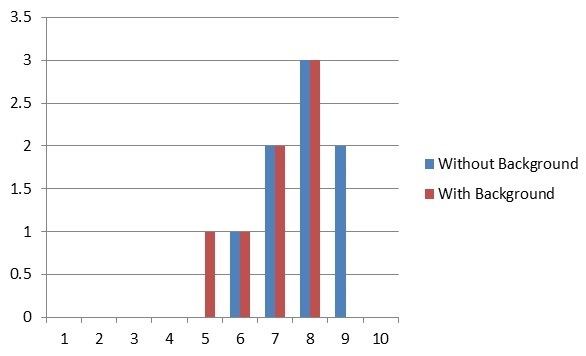
\includegraphics[width = 8.5cm,height = 4.5cm]{images/bargraph2}
   \caption{Bar Graph for the rate of enjoyment of testers.}
   \label{2}
\end{figure}
\newline5.) Would you recommend this game to your friends? \textit{See Fig.8} \newline
-Respondents with no background (Yes - 7, No - 1) \newline
-Respondents with background (Yes - 6, No - 1)\newline
\begin{figure}[ht]
   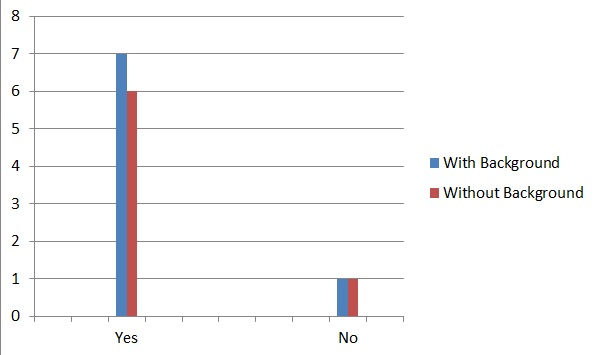
\includegraphics[width = 8.5cm,height = 4cm]{images/bargraph3}
   \caption{Bar Graph for testers who would recommend the game.}
   \label{3}
\end{figure}
\newline
6.) Suggestions on how to improve the game.\newline
-Adjust the camera further \newline
-Option to revisit dialogues \newline
-Add additional levels \newline
-Provide a map for the game \newline
-Fix some bugs

%Discussion
\section{\textbf{Discussion}}
Based from the data given by the respondents, we can say that the game is having a positive effect on the learning experience of the students with regards to programming. Students with no background in programming learned the basic commands in programming provided by the game also, if we compare the students who have a background experience with programming, in terms of rating, they only differ by a little but they both have positive results.\newline
\tab	The game’s aesthetics proved to be not much of a help in a student’s experience because of the “plain” textures that the researcher has provided. However, the score of 7.4 out of 10 in the level of enjoyment is promising despite of the aesthetics being only 5.93 in average. \textit{See Fig. 4}
	When asked if they would recommend the game to their friends, a total of 13 out of 15 respondents \textit{See Fig. 8} said "Yes" and the other 2 responded with "No" which means the success of the game being spread across every students is very highly possible and using the game as one of the source of learning basic programming commands. \newline
\tab	The suggestions prove that there are still improvements that need to be done in order for the game to be fully effective such as: The camera views sometimes go over through walls making players confused on which where they will go. A hint button must be added as well in order for the players to remember the definitions or how some functionality works.


% CONCLUSION AND FUTURE WORK
\section{\textbf{Conclusion and Future Work}}
Overall, the study provided more than average results and it proved to be effective for students with no background in programming to learn the basic programming commands and to learn how to think algorithmically based on the data that were collected. The level of enjoyment of students upon playing the game is satisfactory. The game itself may have some bugs and needs some fixing, in the end, the researcher’s goal has been achieved and that the game will provide good use to students who do not have any background in programming and wants to learn how to program or code.\newline
\tab	For the students who want to follow this study, it is highly recommended that they should improve the aesthetics and fixing bugs in the game since based on the data, the testers have given a low rating for it. More importantly, they need to improve the comprehension methods namely: the visual representation of how the commands work and the actual commands itself.\newline
\tab	Lastly it has proven that, the data given by the testers from the rating of their comprehension for the basic commands and if they would recommend the game to other people, this study is a viable aid in teaching students who are just starting to learn programming and can be a supplementary source for additional understanding of basic programming commands.
\end{justify}

% APPENDICES
%\appendices

%\section{Proof of the First Zonklar Equation}
%Appendix one text goes here...

%\section{}
%Appendix two (without title) text goes here...

% ACKNOWLEDGMENT
\section*{\textbf{Acknowledgment}}
First of all, I would like to thank my adviser for giving me the opportunity to create this Special Problem because this is in-line with my interest as an aspiring game developer. Secondly, I would like to thank my friends and family for their never-ending support. Lastly, Special thanks to Nica Rasco for inspiring and encouraging me to do my best in finishing SP.

% BIBLIOGRAPHY
\bibliographystyle{./IEEE/IEEEtran}
\bibliography{./cs190-ieee}
\nocite{*}

% BIOGRAPHY
%\begin{biography}[{
\includegraphics{./yourPicture.eps}}]{Student M. Name}
%Biography text here...
%\end{biography}


\end{document}
 
